\subsection{Rank lists fusion}
\label{sec:rank_lists_fusion}

The idea of rank list fusion is to combine multiple rank lists in such way that the resulting rank list is more accurate modelization of the real rank list.
The hypotetical best possible approximation of the real rank list in the case of authorship clustering is one such that  every true links (same authors document pairs) are at the top and every false links (different author document pairs) are at the bottom, therefore maximizing every metrics in Section~\ref{sec:rl_eval}.

\subsubsection{Z-Score fusion}

To merge scored rank list with differents order of magnitude, a simple and rather effective approach is to normalize every rank lists scores using the z-score (See Definition~\ref{def:z_score}) and then compute the merge rank list score for every link by taking the arithmetic mean of the same link score for every normalized rank lists.

\textbf{Example with the two rank lists:}

Rank list A (Mean = 50, Std = 40.82):

\begin{tabular}{c l r r}
  \toprule
  Rank & Link name & Score & Z-Score \\
  \midrule
  0 & (0, 1) & $100$ & $1.22$ \\
  1 & (1, 2) & $50$ & $0$ \\
  2 & (0, 2) & $0$ & $-1.22$ \\
  \bottomrule
\end{tabular}

Rank list B (Mean = 0.33, Std = 0.17):

\begin{tabular}{c l r r}
  \toprule
  Rank & Link name & Score & Z-Score \\
  \midrule
  0 & (1, 2) & $0.5$ & $0.98$ \\
  1 & (0, 1) & $0.4$ & $0.39$ \\
  2 & (0, 2) & $0.1$ & $-1.37$ \\
  \bottomrule
\end{tabular}

Z-Score fusion:

\begin{tabular}{c l l}
  \toprule
  Rank & Link name & Average Z-Score \\
  \midrule
  0 & (0, 1) & $(0.39 + 1.22) / 2$ = $0.81$ \\
  1 & (1, 2) & $(0 + 0.98) / 2$ = $0.49$ \\
  2 & (0, 2) & $(-1.22 + -1.37) / 2$ = $-1.30$ \\
  \bottomrule
\end{tabular}

This method can provide good results, but lack of theoretical foundations.

\subsubsection{Regression fusion \label{sec:regression_fusion}}

Each rank list is ordered by a score, this score depends on distance measure used, thus the order of magnitude of each rank list is different.
To avoid having problems in merging rank lists with different magnitude, the solution opted is to translate the scores into a probability of being a true link.
To do so the logistic regression is used.
This method is similar to the one proposed in \textit{Anne Le Calvé and Jacques Savoy (2000)}'s paper~\cite{le_calve_database_merging} and used for merging rank list issued from information retrieval systems.

The main idea here is to learn a logistic regression model for each combination text representation and distance metrics used (here denoted \textit{type of rank list}).
The features used to find the logistic parameters for each link in the rank list are : the log of the relative rank and the link score.
Since a probability of being a true link is desired, the target value for each true link is 1 and 0 when it's a false link.

Once a model per type of rank list is trained, this model can provide for any new same type rank list, probabilities for each link being of being a true link.
The probability framework can now be used on the rank list.
To obtain the most reliable probability given multiple observations (different rank lists), the fusion results in computing the expected value for each link's probability using these observations.
In this case, the expected value is a simple average of the probabilities, since no weighting is used on the rank lists.

\subsubsection{Veto}

To try to improve the results, a veto system is proposed.
The idea here is to have a veto on link with low probatilities.
The following assumption is made: if a link have a low probability in a rank list before the fusion, this probably indicate a false link according to this rank list, thus having theses links at the bottom of the rank list after the fusion can improve the results.

To fullfill the previously stated assumption, a possible way is to find every links in the ranks list before the fusion where the probability is under a certain threshold, and alter this probability with a lower one.
The proposed solution is to set the probability of the affected links (probability of beeing a true link below the threshold) to one of these values : $0$, $-1$, $-n$, $-\infty$, with $n = \#(ranks lists for the fusion)$.
The greater, the value the stronger the penality of the veto.
The $-\infty$ method is the only veto method in the first meaning of the veto definition, every links below the probability will have its final score also equal to $-\infty$ thus in the fused rank list all these links are at the bottom but their order is not defined.

\subsubsection{Soft-veto using S-Curve}

An additional desired constraint is to favor top ranked link and penalize bottom ranked links when fusing rank lists.
This constraint can be easily explained by observing the distance over the rank graph of the rank list.
Figure~\ref{fig:distance_over_rank} clearly show us the top ranked links and bottom ranked links have a sharper decision than in than the middle section.

Top ranked links correspond to similar documents and bottom links correspond to negatively correlated documents.
Assuming that the top rank are true links after the rank list fusion these link should also be top rank.
The same reasoning can be apply for the bottom links by assuming them as false links.
A weighting curve, here called soft-veto, can be design accordingly such that the score of top links are boosted and  bottom links score hindered.

Using the reciprocal of the sigmoid function such curve can modelized.

\begin{equation}
  \label{eq:sigmoid}
  S(x) = \frac{1}{1+e^{-x}}
\end{equation}
\begin{equation}
  \label{eq:sigmoid_r}
  S^{-1}(x) = -\ln{\frac{x-1}{x}}
\end{equation}

The steepness of the curve can be ajusted by changing the start and the end of the interval and then normalizing the values between -1 and 1.
Figure~\ref{fig:s_curve_c} shows the $S^-1(x)$ function normalized between -1 and 1 for the intervals between $\lim\limits_{c \rightarrow 0} \left[S(c), S(c)\right]$ and $\left[S(-20), S(+20)\right]$.
A greater interval size increase the steepness which correspond to an increase of the rank conservation of the top and bottom ranked links and decreasing the rank conservation of the middle ranked links.
To break the symmetry for the curve, to be able to increase the conservation of the top rank while decreasing the conservation of the bottom ranked.
The solution proposed is to add a new parameter $r$, then take $r \cdot N$ samples for $\left[S(-c), S(0)\right]$ and $(1-r) \cdot N$ samples for $\left[S(0), S(c)\right]$.
Figure~\ref{fig:s_curve_r} shows the r parameter influance of a sigmoid with $c = 4$ and $r \in \left[0.1, 0.9\right]$.
The $c$ parameter must be in the interval $\left]0, \infty\right[$, with a value close to $0$ the soft-veto have a weak effect and with a large value, for example 20, the soft veto has a strong effect on the top and bottom, see Figure~\ref{fig:s_curve_c}.
The $r$ parameter must be in the interval $\left]0, 1\right[$, with a value close to $0$ the soft-veto have a strong effect on the top ranked links and with a large value a strong effect on the bottom ranked links, see Figure~\ref{fig:s_curve_r}.

To apply the soft-veto, each score in the rank list is multiplied by the s-curve at the same rank.
This soft-veto methodology aimed to be used on rank list before fusing, to have a more cleaved decision on the links positions.

\begin{figure}
  \centering
  \caption{Distance over rank in the rank list using the smoothed Manhattan distance, 500 MFW tokens on the Brunet dataset}
  \label{fig:distance_over_rank}
  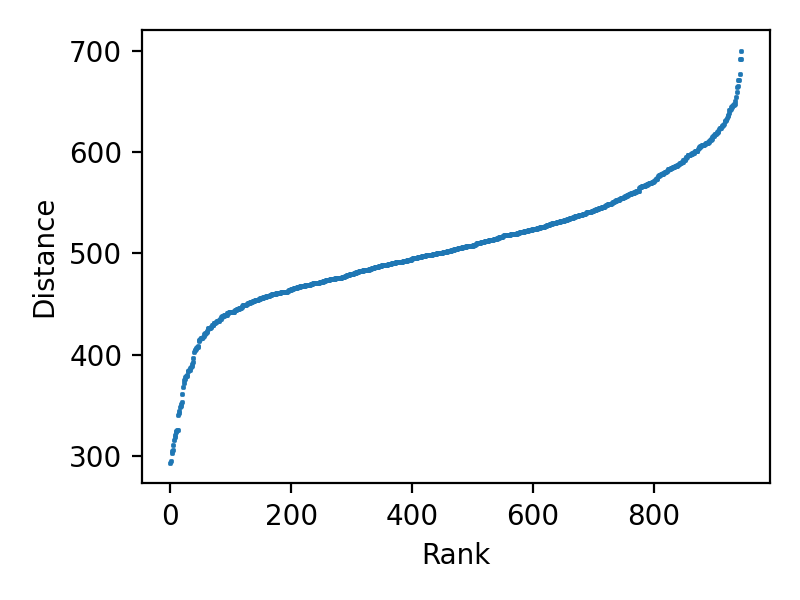
\includegraphics[width=\linewidth]{img/distance_over_rank.png}
\end{figure}


\begin{figure}
  \centering
  \caption{S-Curves parameters}
  \label{fig:s_curve_params}

  \subcaption{$S^-1(x)$, sampled in $\left[S(-c), S(+c)\right]$ and normalized between -1 and 1}
  \label{fig:s_curve_c}
  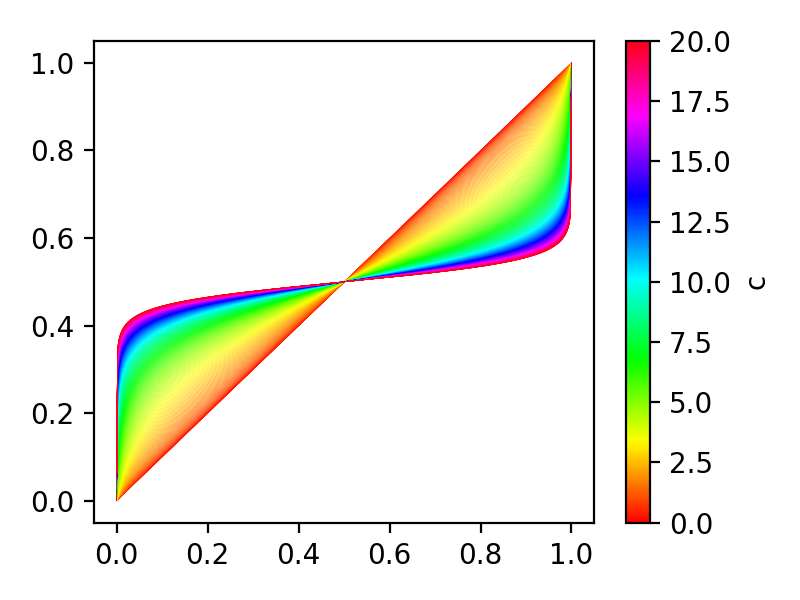
\includegraphics[width=\linewidth]{img/s_curve_c.png}

  \subcaption{Sampling $S^-1(x)$ with $r \cdot N$ samples for $\left[S(-c), S(0)\right]$ and $(1-r) \cdot N$ samples for $\left[S(0), S(c)\right]$}
  \label{fig:s_curve_r}
  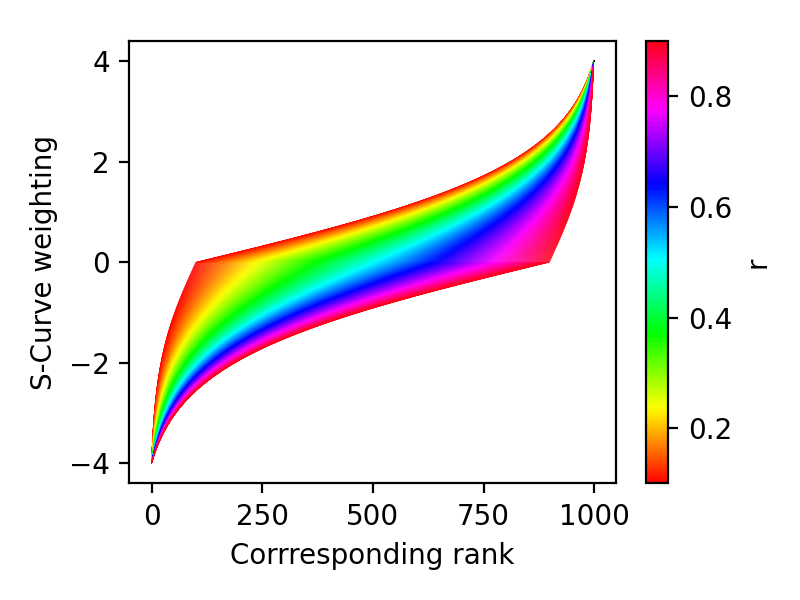
\includegraphics[width=\linewidth]{img/s_curve_r.png}
\end{figure}
